\documentclass[conference]{IEEEtran}
\usepackage{amsmath,amssymb}
\usepackage{fontspec}
\setmainfont{texgyretermes}[Extension=.otf,UprightFont=*-regular,BoldFont=*-bold,ItalicFont=*-italic,BoldItalicFont=*-bolditalic]
\setmonofont{texgyrecursor}[Extension=.otf,UprightFont=*-regular,BoldFont=*-bold,ItalicFont=*-italic,BoldItalicFont=*-bolditalic,Scale=0.95]
\usepackage{graphicx}
\usepackage{booktabs}
\usepackage{cite}
\usepackage{xcolor}
\usepackage{url}
\usepackage[hidelinks]{hyperref}
\newcommand{\NSeeds}{150}
\newcommand{\NFidelity}{6}
\newcommand{\EpisodeTicks}{120}
\newcommand{\DecisionInterval}{10}
\newcommand{\RetryCap}{2}
\newcommand{\Horizon}{20}
\newcommand{\GateTau}{0}
\newcommand{\HarmTheta}{3}
\newcommand{\FaultsPerEpisode}{3}
\newcommand{\FaultStartMin}{20}
\newcommand{\FaultStartMax}{260}
\newcommand{\BootResamples}{5{,}000}
\newcommand{\FaultDurMin}{20}
\newcommand{\FaultDurMax}{80}
\newcommand{\SwitchThreshold}{0.5}
\newcommand{\EpisodesPerCondition}{3{,}150}
\newcommand{\EpisodesTotal}{6{,}300}
\newcommand{\RandomGatePRule}{0.30}
\newcommand{\RandomGatePScr}{0.747}
\newcommand{\BaselineTicks}{122.1}
\newcommand{\RuleNetZeroI}{\ensuremath{-}0.147}
\newcommand{\RuleNetCIZeroI}{[\ensuremath{-}0.627, \ensuremath{+}0.313]}
\newcommand{\RuleBPZeroI}{0.409}
\newcommand{\RuleHPZeroI}{0.747}
\newcommand{\RuleEpZeroI}{\ensuremath{+}1.073}
\newcommand{\RuleEpCIZeroI}{[\ensuremath{-}0.048, \ensuremath{+}2.194]}
\newcommand{\RuleEpPZeroI}{0.011}
\newcommand{\RuleEpHolmZeroI}{0.066}
\newcommand{\RuleEpNZZeroI}{29}
\newcommand{\RuleEpBetterZeroI}{6}
\newcommand{\RuleEpWorseZeroI}{23}
\newcommand{\RuleEpPowerZeroI}{0.73}
\newcommand{\RuleEpNeedZeroI}{329}
\newcommand{\RuleNetTwoI}{\ensuremath{-}0.393}
\newcommand{\RuleNetCITwoI}{[\ensuremath{-}0.800, \ensuremath{-}0.027]}
\newcommand{\RuleBPTwoI}{0.431}
\newcommand{\RuleHPTwoI}{0.818}
\newcommand{\RuleEpTwoI}{\ensuremath{+}0.760}
\newcommand{\RuleEpCITwoI}{[\ensuremath{-}0.356, \ensuremath{+}1.876]}
\newcommand{\RuleEpPTwoI}{0.111}
\newcommand{\RuleEpHolmTwoI}{0.556}
\newcommand{\RuleEpNZTwoI}{25}
\newcommand{\RuleEpBetterTwoI}{8}
\newcommand{\RuleEpWorseTwoI}{17}
\newcommand{\RuleEpPowerTwoI}{0.36}
\newcommand{\RuleEpNeedTwoI}{651}
\newcommand{\RuleNetFourI}{\ensuremath{-}0.593}
\newcommand{\RuleNetCIFourI}{[\ensuremath{-}1.127, \ensuremath{-}0.113]}
\newcommand{\RuleBPFourI}{0.373}
\newcommand{\RuleHPFourI}{0.926}
\newcommand{\RuleEpFourI}{\ensuremath{-}0.500}
\newcommand{\RuleEpCIFourI}{[\ensuremath{-}1.518, \ensuremath{+}0.518]}
\newcommand{\RuleEpPFourI}{0.411}
\newcommand{\RuleEpHolmFourI}{0.822}
\newcommand{\RuleEpNZFourI}{16}
\newcommand{\RuleEpBetterFourI}{10}
\newcommand{\RuleEpWorseFourI}{6}
\newcommand{\RuleEpPowerFourI}{0.13}
\newcommand{\RuleEpNeedFourI}{1{,}251}
\newcommand{\RuleNetSixI}{\ensuremath{-}0.780}
\newcommand{\RuleNetCISixI}{[\ensuremath{-}1.273, \ensuremath{-}0.360]}
\newcommand{\RuleBPSixI}{0.424}
\newcommand{\RuleHPSixI}{0.965}
\newcommand{\RuleEpSixI}{\ensuremath{-}1.067}
\newcommand{\RuleEpCISixI}{[\ensuremath{-}2.167, \ensuremath{+}0.034]}
\newcommand{\RuleEpPSixI}{0.117}
\newcommand{\RuleEpHolmSixI}{0.556}
\newcommand{\RuleEpNZSixI}{17}
\newcommand{\RuleEpBetterSixI}{11}
\newcommand{\RuleEpWorseSixI}{6}
\newcommand{\RuleEpPowerSixI}{0.32}
\newcommand{\RuleEpNeedSixI}{322}
\newcommand{\RuleNetEightI}{\ensuremath{-}1.320}
\newcommand{\RuleNetCIEightI}{[\ensuremath{-}2.107, \ensuremath{-}0.653]}
\newcommand{\RuleBPEightI}{0.609}
\newcommand{\RuleHPEightI}{0.989}
\newcommand{\RuleEpEightI}{\ensuremath{-}1.707}
\newcommand{\RuleEpCIEightI}{[\ensuremath{-}2.987, \ensuremath{-}0.426]}
\newcommand{\RuleEpPEightI}{0.0036}
\newcommand{\RuleEpHolmEightI}{0.025}
\newcommand{\RuleEpNZEightI}{18}
\newcommand{\RuleEpBetterEightI}{15}
\newcommand{\RuleEpWorseEightI}{3}
\newcommand{\RuleEpPowerEightI}{0.87}
\newcommand{\RuleEpNeedEightI}{170}
\newcommand{\RuleNetTenI}{\ensuremath{-}2.120}
\newcommand{\RuleNetCITenI}{[\ensuremath{-}3.240, \ensuremath{-}1.093]}
\newcommand{\RuleBPTenI}{0.970}
\newcommand{\RuleHPTenI}{0.991}
\newcommand{\RuleEpTenI}{\ensuremath{-}2.320}
\newcommand{\RuleEpCITenI}{[\ensuremath{-}3.762, \ensuremath{-}0.878]}
\newcommand{\RuleEpPTenI}{\ensuremath{9.7\times 10^{-4}}}
\newcommand{\RuleEpHolmTenI}{0.0078}
\newcommand{\RuleEpNZTenI}{22}
\newcommand{\RuleEpBetterTenI}{18}
\newcommand{\RuleEpWorseTenI}{4}
\newcommand{\RuleEpPowerTenI}{0.96}
\newcommand{\RuleEpNeedTenI}{117}
\newcommand{\RuleCrossNI}{0}
\newcommand{\RuleMonotoneI}{yes}
\newcommand{\RuleUngatedEpI}{\ensuremath{+}3.393}
\newcommand{\RuleUngatedEpCII}{[\ensuremath{+}1.338, \ensuremath{+}5.449]}
\newcommand{\RuleUngatedEpPI}{\ensuremath{1.2\times 10^{-4}}}
\newcommand{\RuleUngatedEpHolmI}{0.0011}
\newcommand{\RuleUngatedEpNZI}{71}
\newcommand{\RuleUngatedEpBetterI}{14}
\newcommand{\RuleUngatedEpWorseI}{57}
\newcommand{\RuleRandomEpI}{\ensuremath{+}3.327}
\newcommand{\RuleRandomEpCII}{[\ensuremath{+}1.366, \ensuremath{+}5.287]}
\newcommand{\RuleRandomEpPI}{\ensuremath{6.8\times 10^{-5}}}
\newcommand{\RuleRandomEpHolmI}{\ensuremath{7.5\times 10^{-4}}}
\newcommand{\RuleRandomEpNZI}{63}
\newcommand{\RuleRandomEpBetterI}{13}
\newcommand{\RuleRandomEpWorseI}{50}
\newcommand{\RuleOracleEpI}{\ensuremath{-}2.587}
\newcommand{\RuleOracleEpCII}{[\ensuremath{-}4.027, \ensuremath{-}1.146]}
\newcommand{\RuleOracleEpPI}{\ensuremath{8.3\times 10^{-5}}}
\newcommand{\RuleOracleEpHolmI}{\ensuremath{8.3\times 10^{-4}}}
\newcommand{\RuleOracleEpNZI}{22}
\newcommand{\RuleOracleEpBetterI}{20}
\newcommand{\RuleOracleEpWorseI}{2}
\newcommand{\RuleTenVsZeroEpI}{\ensuremath{-}3.393}
\newcommand{\RuleTenVsZeroEpCII}{[\ensuremath{-}5.018, \ensuremath{-}1.768]}
\newcommand{\RuleTenVsZeroEpPI}{\ensuremath{9.2\times 10^{-7}}}
\newcommand{\RuleTenVsZeroEpHolmI}{\ensuremath{1.1\times 10^{-5}}}
\newcommand{\RuleTenVsZeroEpNZI}{38}
\newcommand{\RuleTenVsZeroEpBetterI}{33}
\newcommand{\RuleTenVsZeroEpWorseI}{5}
\newcommand{\RuleRejAvailBenefitI}{439}
\newcommand{\RuleRejAvailBenefitPerSeedI}{2.93}
\newcommand{\RuleRejSeedsBenefitI}{23}
\newcommand{\RuleRejBeneficialI}{48}
\newcommand{\RuleRejHarmfulAboveThreeI}{91}
\newcommand{\RuleAnyArmSeedsBenefitI}{59}
\newcommand{\RuleRejEpMeanI}{122.1}
\newcommand{\RuleNetZeroII}{\ensuremath{-}0.127}
\newcommand{\RuleNetCIZeroII}{[\ensuremath{-}0.633, \ensuremath{+}0.387]}
\newcommand{\RuleBPZeroII}{0.430}
\newcommand{\RuleHPZeroII}{0.737}
\newcommand{\RuleEpZeroII}{\ensuremath{+}0.973}
\newcommand{\RuleEpCIZeroII}{[\ensuremath{-}0.053, \ensuremath{+}2.000]}
\newcommand{\RuleEpPZeroII}{0.015}
\newcommand{\RuleEpHolmZeroII}{0.088}
\newcommand{\RuleEpNZZeroII}{28}
\newcommand{\RuleEpBetterZeroII}{6}
\newcommand{\RuleEpWorseZeroII}{22}
\newcommand{\RuleEpPowerZeroII}{0.68}
\newcommand{\RuleEpNeedZeroII}{336}
\newcommand{\RuleNetTwoII}{\ensuremath{-}0.447}
\newcommand{\RuleNetCITwoII}{[\ensuremath{-}0.913, \ensuremath{+}0.000]}
\newcommand{\RuleBPTwoII}{0.349}
\newcommand{\RuleHPTwoII}{0.886}
\newcommand{\RuleEpTwoII}{\ensuremath{-}0.140}
\newcommand{\RuleEpCITwoII}{[\ensuremath{-}1.152, \ensuremath{+}0.872]}
\newcommand{\RuleEpPTwoII}{0.977}
\newcommand{\RuleEpHolmTwoII}{1.000}
\newcommand{\RuleEpNZTwoII}{19}
\newcommand{\RuleEpBetterTwoII}{10}
\newcommand{\RuleEpWorseTwoII}{9}
\newcommand{\RuleEpPowerTwoII}{0.04}
\newcommand{\RuleEpNeedTwoII}{15{,}761}
\newcommand{\RuleNetFourII}{\ensuremath{-}0.787}
\newcommand{\RuleNetCIFourII}{[\ensuremath{-}1.307, \ensuremath{-}0.347]}
\newcommand{\RuleBPFourII}{0.482}
\newcommand{\RuleHPFourII}{0.928}
\newcommand{\RuleEpFourII}{\ensuremath{-}0.767}
\newcommand{\RuleEpCIFourII}{[\ensuremath{-}1.968, \ensuremath{+}0.434]}
\newcommand{\RuleEpPFourII}{0.474}
\newcommand{\RuleEpHolmFourII}{1.000}
\newcommand{\RuleEpNZFourII}{18}
\newcommand{\RuleEpBetterFourII}{10}
\newcommand{\RuleEpWorseFourII}{8}
\newcommand{\RuleEpPowerFourII}{0.10}
\newcommand{\RuleEpNeedFourII}{740}
\newcommand{\RuleNetSixII}{\ensuremath{-}0.780}
\newcommand{\RuleNetCISixII}{[\ensuremath{-}1.273, \ensuremath{-}0.360]}
\newcommand{\RuleBPSixII}{0.424}
\newcommand{\RuleHPSixII}{0.965}
\newcommand{\RuleEpSixII}{\ensuremath{-}1.067}
\newcommand{\RuleEpCISixII}{[\ensuremath{-}2.167, \ensuremath{+}0.034]}
\newcommand{\RuleEpPSixII}{0.117}
\newcommand{\RuleEpHolmSixII}{0.583}
\newcommand{\RuleEpNZSixII}{17}
\newcommand{\RuleEpBetterSixII}{11}
\newcommand{\RuleEpWorseSixII}{6}
\newcommand{\RuleEpPowerSixII}{0.32}
\newcommand{\RuleEpNeedSixII}{322}
\newcommand{\RuleNetEightII}{\ensuremath{-}1.320}
\newcommand{\RuleNetCIEightII}{[\ensuremath{-}2.107, \ensuremath{-}0.653]}
\newcommand{\RuleBPEightII}{0.609}
\newcommand{\RuleHPEightII}{0.989}
\newcommand{\RuleEpEightII}{\ensuremath{-}1.707}
\newcommand{\RuleEpCIEightII}{[\ensuremath{-}2.987, \ensuremath{-}0.426]}
\newcommand{\RuleEpPEightII}{0.0036}
\newcommand{\RuleEpHolmEightII}{0.025}
\newcommand{\RuleEpNZEightII}{18}
\newcommand{\RuleEpBetterEightII}{15}
\newcommand{\RuleEpWorseEightII}{3}
\newcommand{\RuleEpPowerEightII}{0.87}
\newcommand{\RuleEpNeedEightII}{170}
\newcommand{\RuleNetTenII}{\ensuremath{-}2.120}
\newcommand{\RuleNetCITenII}{[\ensuremath{-}3.240, \ensuremath{-}1.093]}
\newcommand{\RuleBPTenII}{0.970}
\newcommand{\RuleHPTenII}{0.991}
\newcommand{\RuleEpTenII}{\ensuremath{-}2.320}
\newcommand{\RuleEpCITenII}{[\ensuremath{-}3.762, \ensuremath{-}0.878]}
\newcommand{\RuleEpPTenII}{\ensuremath{9.7\times 10^{-4}}}
\newcommand{\RuleEpHolmTenII}{0.0078}
\newcommand{\RuleEpNZTenII}{22}
\newcommand{\RuleEpBetterTenII}{18}
\newcommand{\RuleEpWorseTenII}{4}
\newcommand{\RuleEpPowerTenII}{0.96}
\newcommand{\RuleEpNeedTenII}{117}
\newcommand{\RuleCrossNII}{0}
\newcommand{\RuleMonotoneII}{no}
\newcommand{\RuleUngatedEpII}{\ensuremath{+}3.393}
\newcommand{\RuleUngatedEpCIII}{[\ensuremath{+}1.338, \ensuremath{+}5.449]}
\newcommand{\RuleUngatedEpPII}{\ensuremath{1.2\times 10^{-4}}}
\newcommand{\RuleUngatedEpHolmII}{0.0011}
\newcommand{\RuleUngatedEpNZII}{71}
\newcommand{\RuleUngatedEpBetterII}{14}
\newcommand{\RuleUngatedEpWorseII}{57}
\newcommand{\RuleRandomEpII}{\ensuremath{+}3.327}
\newcommand{\RuleRandomEpCIII}{[\ensuremath{+}1.366, \ensuremath{+}5.287]}
\newcommand{\RuleRandomEpPII}{\ensuremath{6.8\times 10^{-5}}}
\newcommand{\RuleRandomEpHolmII}{\ensuremath{7.5\times 10^{-4}}}
\newcommand{\RuleRandomEpNZII}{63}
\newcommand{\RuleRandomEpBetterII}{13}
\newcommand{\RuleRandomEpWorseII}{50}
\newcommand{\RuleOracleEpII}{\ensuremath{-}2.587}
\newcommand{\RuleOracleEpCIII}{[\ensuremath{-}4.027, \ensuremath{-}1.146]}
\newcommand{\RuleOracleEpPII}{\ensuremath{8.3\times 10^{-5}}}
\newcommand{\RuleOracleEpHolmII}{\ensuremath{8.3\times 10^{-4}}}
\newcommand{\RuleOracleEpNZII}{22}
\newcommand{\RuleOracleEpBetterII}{20}
\newcommand{\RuleOracleEpWorseII}{2}
\newcommand{\RuleTenVsZeroEpII}{\ensuremath{-}3.293}
\newcommand{\RuleTenVsZeroEpCIII}{[\ensuremath{-}4.910, \ensuremath{-}1.677]}
\newcommand{\RuleTenVsZeroEpPII}{\ensuremath{9.1\times 10^{-7}}}
\newcommand{\RuleTenVsZeroEpHolmII}{\ensuremath{1.1\times 10^{-5}}}
\newcommand{\RuleTenVsZeroEpNZII}{37}
\newcommand{\RuleTenVsZeroEpBetterII}{32}
\newcommand{\RuleTenVsZeroEpWorseII}{5}
\newcommand{\RuleRejAvailBenefitII}{439}
\newcommand{\RuleRejAvailBenefitPerSeedII}{2.93}
\newcommand{\RuleRejSeedsBenefitII}{23}
\newcommand{\RuleRejBeneficialII}{48}
\newcommand{\RuleRejHarmfulAboveThreeII}{91}
\newcommand{\RuleAnyArmSeedsBenefitII}{59}
\newcommand{\RuleRejEpMeanII}{122.1}
\newcommand{\ScrNetZeroI}{\ensuremath{+}3.033}
\newcommand{\ScrNetCIZeroI}{[\ensuremath{+}2.173, \ensuremath{+}3.893]}
\newcommand{\ScrBPZeroI}{0.727}
\newcommand{\ScrHPZeroI}{0.681}
\newcommand{\ScrEpZeroI}{\ensuremath{+}15.013}
\newcommand{\ScrEpCIZeroI}{[\ensuremath{+}12.847, \ensuremath{+}17.179]}
\newcommand{\ScrEpPZeroI}{\ensuremath{2.1\times 10^{-37}}}
\newcommand{\ScrEpHolmZeroI}{\ensuremath{1.9\times 10^{-36}}}
\newcommand{\ScrEpNZZeroI}{128}
\newcommand{\ScrEpBetterZeroI}{2}
\newcommand{\ScrEpWorseZeroI}{126}
\newcommand{\ScrEpPowerZeroI}{1.00}
\newcommand{\ScrEpNeedZeroI}{7}
\newcommand{\ScrNetTwoI}{\ensuremath{+}2.413}
\newcommand{\ScrNetCITwoI}{[\ensuremath{+}1.567, \ensuremath{+}3.267]}
\newcommand{\ScrBPTwoI}{0.803}
\newcommand{\ScrHPTwoI}{0.755}
\newcommand{\ScrEpTwoI}{\ensuremath{+}11.280}
\newcommand{\ScrEpCITwoI}{[\ensuremath{+}9.449, \ensuremath{+}13.111]}
\newcommand{\ScrEpPTwoI}{\ensuremath{6.0\times 10^{-36}}}
\newcommand{\ScrEpHolmTwoI}{\ensuremath{4.8\times 10^{-35}}}
\newcommand{\ScrEpNZTwoI}{122}
\newcommand{\ScrEpBetterTwoI}{2}
\newcommand{\ScrEpWorseTwoI}{120}
\newcommand{\ScrEpPowerTwoI}{1.00}
\newcommand{\ScrEpNeedTwoI}{8}
\newcommand{\ScrNetFourI}{\ensuremath{+}0.987}
\newcommand{\ScrNetCIFourI}{[\ensuremath{+}0.347, \ensuremath{+}1.653]}
\newcommand{\ScrBPFourI}{0.819}
\newcommand{\ScrHPFourI}{0.870}
\newcommand{\ScrEpFourI}{\ensuremath{+}6.313}
\newcommand{\ScrEpCIFourI}{[\ensuremath{+}4.722, \ensuremath{+}7.905]}
\newcommand{\ScrEpPFourI}{\ensuremath{7.7\times 10^{-22}}}
\newcommand{\ScrEpHolmFourI}{\ensuremath{5.4\times 10^{-21}}}
\newcommand{\ScrEpNZFourI}{84}
\newcommand{\ScrEpBetterFourI}{4}
\newcommand{\ScrEpWorseFourI}{80}
\newcommand{\ScrEpPowerFourI}{1.00}
\newcommand{\ScrEpNeedFourI}{20}
\newcommand{\ScrNetSixI}{\ensuremath{-}0.287}
\newcommand{\ScrNetCISixI}{[\ensuremath{-}0.807, \ensuremath{+}0.213]}
\newcommand{\ScrBPSixI}{0.839}
\newcommand{\ScrHPSixI}{0.962}
\newcommand{\ScrEpSixI}{\ensuremath{+}2.367}
\newcommand{\ScrEpCISixI}{[\ensuremath{+}1.231, \ensuremath{+}3.502]}
\newcommand{\ScrEpPSixI}{\ensuremath{2.2\times 10^{-9}}}
\newcommand{\ScrEpHolmSixI}{\ensuremath{1.3\times 10^{-8}}}
\newcommand{\ScrEpNZSixI}{42}
\newcommand{\ScrEpBetterSixI}{7}
\newcommand{\ScrEpWorseSixI}{35}
\newcommand{\ScrEpPowerSixI}{1.00}
\newcommand{\ScrEpNeedSixI}{70}
\newcommand{\ScrNetEightI}{\ensuremath{-}0.587}
\newcommand{\ScrNetCIEightI}{[\ensuremath{-}1.027, \ensuremath{-}0.193]}
\newcommand{\ScrBPEightI}{0.901}
\newcommand{\ScrHPEightI}{0.990}
\newcommand{\ScrEpEightI}{\ensuremath{+}0.560}
\newcommand{\ScrEpCIEightI}{[\ensuremath{+}0.090, \ensuremath{+}1.030]}
\newcommand{\ScrEpPEightI}{0.0097}
\newcommand{\ScrEpHolmEightI}{0.049}
\newcommand{\ScrEpNZEightI}{23}
\newcommand{\ScrEpBetterEightI}{6}
\newcommand{\ScrEpWorseEightI}{17}
\newcommand{\ScrEpPowerEightI}{0.72}
\newcommand{\ScrEpNeedEightI}{213}
\newcommand{\ScrNetTenI}{\ensuremath{-}0.620}
\newcommand{\ScrNetCITenI}{[\ensuremath{-}1.027, \ensuremath{-}0.253]}
\newcommand{\ScrBPTenI}{0.877}
\newcommand{\ScrHPTenI}{0.994}
\newcommand{\ScrEpTenI}{\ensuremath{+}0.233}
\newcommand{\ScrEpCITenI}{[\ensuremath{-}0.156, \ensuremath{+}0.622]}
\newcommand{\ScrEpPTenI}{0.287}
\newcommand{\ScrEpHolmTenI}{0.574}
\newcommand{\ScrEpNZTenI}{17}
\newcommand{\ScrEpBetterTenI}{7}
\newcommand{\ScrEpWorseTenI}{10}
\newcommand{\ScrEpPowerTenI}{0.21}
\newcommand{\ScrEpNeedTenI}{839}
\newcommand{\ScrCrossNI}{1}
\newcommand{\ScrCrossI}{0.555}
\newcommand{\ScrCrossCII}{[0.471, 0.677]}
\newcommand{\ScrCrossSingleI}{4{,}997}
\newcommand{\ScrMonotoneI}{yes}
\newcommand{\ScrUngatedEpI}{\ensuremath{+}25.060}
\newcommand{\ScrUngatedEpCII}{[\ensuremath{+}22.320, \ensuremath{+}27.800]}
\newcommand{\ScrUngatedEpPI}{\ensuremath{2.8\times 10^{-45}}}
\newcommand{\ScrUngatedEpHolmI}{\ensuremath{3.4\times 10^{-44}}}
\newcommand{\ScrUngatedEpNZI}{149}
\newcommand{\ScrUngatedEpBetterI}{0}
\newcommand{\ScrUngatedEpWorseI}{149}
\newcommand{\ScrRandomEpI}{\ensuremath{+}20.180}
\newcommand{\ScrRandomEpCII}{[\ensuremath{+}17.441, \ensuremath{+}22.919]}
\newcommand{\ScrRandomEpPI}{\ensuremath{2.9\times 10^{-38}}}
\newcommand{\ScrRandomEpHolmI}{\ensuremath{3.2\times 10^{-37}}}
\newcommand{\ScrRandomEpNZI}{132}
\newcommand{\ScrRandomEpBetterI}{3}
\newcommand{\ScrRandomEpWorseI}{129}
\newcommand{\ScrOracleEpI}{\ensuremath{-}0.213}
\newcommand{\ScrOracleEpCII}{[\ensuremath{-}0.607, \ensuremath{+}0.180]}
\newcommand{\ScrOracleEpPI}{0.087}
\newcommand{\ScrOracleEpHolmI}{0.262}
\newcommand{\ScrOracleEpNZI}{18}
\newcommand{\ScrOracleEpBetterI}{12}
\newcommand{\ScrOracleEpWorseI}{6}
\newcommand{\ScrTenVsZeroEpI}{\ensuremath{-}14.780}
\newcommand{\ScrTenVsZeroEpCII}{[\ensuremath{-}16.988, \ensuremath{-}12.572]}
\newcommand{\ScrTenVsZeroEpPI}{\ensuremath{1.9\times 10^{-37}}}
\newcommand{\ScrTenVsZeroEpHolmI}{\ensuremath{1.9\times 10^{-36}}}
\newcommand{\ScrTenVsZeroEpNZI}{127}
\newcommand{\ScrTenVsZeroEpBetterI}{125}
\newcommand{\ScrTenVsZeroEpWorseI}{2}
\newcommand{\ScrRejAvailBenefitI}{52}
\newcommand{\ScrRejAvailBenefitPerSeedI}{0.35}
\newcommand{\ScrRejSeedsBenefitI}{12}
\newcommand{\ScrRejBeneficialI}{15}
\newcommand{\ScrRejHarmfulAboveThreeI}{922}
\newcommand{\ScrAnyArmSeedsBenefitI}{149}
\newcommand{\ScrRejEpMeanI}{122.1}
\newcommand{\ScrNetZeroII}{\ensuremath{+}2.227}
\newcommand{\ScrNetCIZeroII}{[\ensuremath{+}1.367, \ensuremath{+}3.100]}
\newcommand{\ScrBPZeroII}{0.751}
\newcommand{\ScrHPZeroII}{0.710}
\newcommand{\ScrEpZeroII}{\ensuremath{+}12.433}
\newcommand{\ScrEpCIZeroII}{[\ensuremath{+}10.550, \ensuremath{+}14.316]}
\newcommand{\ScrEpPZeroII}{\ensuremath{1.5\times 10^{-34}}}
\newcommand{\ScrEpHolmZeroII}{\ensuremath{1.5\times 10^{-33}}}
\newcommand{\ScrEpNZZeroII}{130}
\newcommand{\ScrEpBetterZeroII}{4}
\newcommand{\ScrEpWorseZeroII}{126}
\newcommand{\ScrEpPowerZeroII}{1.00}
\newcommand{\ScrEpNeedZeroII}{7}
\newcommand{\ScrNetTwoII}{\ensuremath{+}1.787}
\newcommand{\ScrNetCITwoII}{[\ensuremath{+}0.920, \ensuremath{+}2.613]}
\newcommand{\ScrBPTwoII}{0.772}
\newcommand{\ScrHPTwoII}{0.783}
\newcommand{\ScrEpTwoII}{\ensuremath{+}10.580}
\newcommand{\ScrEpCITwoII}{[\ensuremath{+}8.623, \ensuremath{+}12.537]}
\newcommand{\ScrEpPTwoII}{\ensuremath{2.2\times 10^{-32}}}
\newcommand{\ScrEpHolmTwoII}{\ensuremath{1.8\times 10^{-31}}}
\newcommand{\ScrEpNZTwoII}{115}
\newcommand{\ScrEpBetterTwoII}{3}
\newcommand{\ScrEpWorseTwoII}{112}
\newcommand{\ScrEpPowerTwoII}{1.00}
\newcommand{\ScrEpNeedTwoII}{11}
\newcommand{\ScrNetFourII}{\ensuremath{+}0.827}
\newcommand{\ScrNetCIFourII}{[\ensuremath{+}0.133, \ensuremath{+}1.560]}
\newcommand{\ScrBPFourII}{0.802}
\newcommand{\ScrHPFourII}{0.874}
\newcommand{\ScrEpFourII}{\ensuremath{+}6.167}
\newcommand{\ScrEpCIFourII}{[\ensuremath{+}4.592, \ensuremath{+}7.741]}
\newcommand{\ScrEpPFourII}{\ensuremath{4.1\times 10^{-22}}}
\newcommand{\ScrEpHolmFourII}{\ensuremath{2.9\times 10^{-21}}}
\newcommand{\ScrEpNZFourII}{86}
\newcommand{\ScrEpBetterFourII}{7}
\newcommand{\ScrEpWorseFourII}{79}
\newcommand{\ScrEpPowerFourII}{1.00}
\newcommand{\ScrEpNeedFourII}{20}
\newcommand{\ScrNetSixII}{\ensuremath{-}0.287}
\newcommand{\ScrNetCISixII}{[\ensuremath{-}0.807, \ensuremath{+}0.213]}
\newcommand{\ScrBPSixII}{0.839}
\newcommand{\ScrHPSixII}{0.962}
\newcommand{\ScrEpSixII}{\ensuremath{+}2.367}
\newcommand{\ScrEpCISixII}{[\ensuremath{+}1.231, \ensuremath{+}3.502]}
\newcommand{\ScrEpPSixII}{\ensuremath{2.2\times 10^{-9}}}
\newcommand{\ScrEpHolmSixII}{\ensuremath{1.3\times 10^{-8}}}
\newcommand{\ScrEpNZSixII}{42}
\newcommand{\ScrEpBetterSixII}{7}
\newcommand{\ScrEpWorseSixII}{35}
\newcommand{\ScrEpPowerSixII}{1.00}
\newcommand{\ScrEpNeedSixII}{70}
\newcommand{\ScrNetEightII}{\ensuremath{-}0.587}
\newcommand{\ScrNetCIEightII}{[\ensuremath{-}1.027, \ensuremath{-}0.193]}
\newcommand{\ScrBPEightII}{0.901}
\newcommand{\ScrHPEightII}{0.990}
\newcommand{\ScrEpEightII}{\ensuremath{+}0.560}
\newcommand{\ScrEpCIEightII}{[\ensuremath{+}0.090, \ensuremath{+}1.030]}
\newcommand{\ScrEpPEightII}{0.0097}
\newcommand{\ScrEpHolmEightII}{0.049}
\newcommand{\ScrEpNZEightII}{23}
\newcommand{\ScrEpBetterEightII}{6}
\newcommand{\ScrEpWorseEightII}{17}
\newcommand{\ScrEpPowerEightII}{0.72}
\newcommand{\ScrEpNeedEightII}{213}
\newcommand{\ScrNetTenII}{\ensuremath{-}0.620}
\newcommand{\ScrNetCITenII}{[\ensuremath{-}1.027, \ensuremath{-}0.253]}
\newcommand{\ScrBPTenII}{0.877}
\newcommand{\ScrHPTenII}{0.994}
\newcommand{\ScrEpTenII}{\ensuremath{+}0.233}
\newcommand{\ScrEpCITenII}{[\ensuremath{-}0.156, \ensuremath{+}0.622]}
\newcommand{\ScrEpPTenII}{0.287}
\newcommand{\ScrEpHolmTenII}{0.574}
\newcommand{\ScrEpNZTenII}{17}
\newcommand{\ScrEpBetterTenII}{7}
\newcommand{\ScrEpWorseTenII}{10}
\newcommand{\ScrEpPowerTenII}{0.21}
\newcommand{\ScrEpNeedTenII}{839}
\newcommand{\ScrCrossNII}{1}
\newcommand{\ScrCrossII}{0.549}
\newcommand{\ScrCrossCIII}{[0.434, 0.677]}
\newcommand{\ScrCrossSingleII}{4{,}997}
\newcommand{\ScrMonotoneII}{yes}
\newcommand{\ScrUngatedEpII}{\ensuremath{+}25.060}
\newcommand{\ScrUngatedEpCIII}{[\ensuremath{+}22.320, \ensuremath{+}27.800]}
\newcommand{\ScrUngatedEpPII}{\ensuremath{2.8\times 10^{-45}}}
\newcommand{\ScrUngatedEpHolmII}{\ensuremath{3.4\times 10^{-44}}}
\newcommand{\ScrUngatedEpNZII}{149}
\newcommand{\ScrUngatedEpBetterII}{0}
\newcommand{\ScrUngatedEpWorseII}{149}
\newcommand{\ScrRandomEpII}{\ensuremath{+}20.180}
\newcommand{\ScrRandomEpCIII}{[\ensuremath{+}17.441, \ensuremath{+}22.919]}
\newcommand{\ScrRandomEpPII}{\ensuremath{2.9\times 10^{-38}}}
\newcommand{\ScrRandomEpHolmII}{\ensuremath{3.2\times 10^{-37}}}
\newcommand{\ScrRandomEpNZII}{132}
\newcommand{\ScrRandomEpBetterII}{3}
\newcommand{\ScrRandomEpWorseII}{129}
\newcommand{\ScrOracleEpII}{\ensuremath{-}0.213}
\newcommand{\ScrOracleEpCIII}{[\ensuremath{-}0.607, \ensuremath{+}0.180]}
\newcommand{\ScrOracleEpPII}{0.087}
\newcommand{\ScrOracleEpHolmII}{0.262}
\newcommand{\ScrOracleEpNZII}{18}
\newcommand{\ScrOracleEpBetterII}{12}
\newcommand{\ScrOracleEpWorseII}{6}
\newcommand{\ScrTenVsZeroEpII}{\ensuremath{-}12.200}
\newcommand{\ScrTenVsZeroEpCIII}{[\ensuremath{-}14.095, \ensuremath{-}10.305]}
\newcommand{\ScrTenVsZeroEpPII}{\ensuremath{1.4\times 10^{-33}}}
\newcommand{\ScrTenVsZeroEpHolmII}{\ensuremath{1.3\times 10^{-32}}}
\newcommand{\ScrTenVsZeroEpNZII}{128}
\newcommand{\ScrTenVsZeroEpBetterII}{123}
\newcommand{\ScrTenVsZeroEpWorseII}{5}
\newcommand{\ScrRejAvailBenefitII}{52}
\newcommand{\ScrRejAvailBenefitPerSeedII}{0.35}
\newcommand{\ScrRejSeedsBenefitII}{12}
\newcommand{\ScrRejBeneficialII}{15}
\newcommand{\ScrRejHarmfulAboveThreeII}{922}
\newcommand{\ScrAnyArmSeedsBenefitII}{149}
\newcommand{\ScrRejEpMeanII}{122.1}
\newcommand{\RuleStepFourSixII}{\ensuremath{+}0.007}
\newcommand{\RuleStepFourSixCIII}{[\ensuremath{-}0.133, \ensuremath{+}0.193]}
\newcommand{\RuleSwitchFour}{\ensuremath{-}0.193}
\newcommand{\RuleSwitchFourCI}{[\ensuremath{-}0.513, \ensuremath{+}0.040]}
\newcommand{\RuleSwitchFourP}{0.27}
\newcommand{\RuleSwitchZero}{\ensuremath{+}0.020}
\newcommand{\RuleIdenticalArms}{7}
\newcommand{\ScrStepFourSixII}{\ensuremath{-}1.113}
\newcommand{\ScrStepFourSixCIII}{[\ensuremath{-}1.753, \ensuremath{-}0.507]}
\newcommand{\ScrSwitchFour}{\ensuremath{-}0.160}
\newcommand{\ScrSwitchFourCI}{[\ensuremath{-}0.813, \ensuremath{+}0.480]}
\newcommand{\ScrSwitchFourP}{0.61}
\newcommand{\ScrSwitchZero}{\ensuremath{-}0.807}
\newcommand{\ScrIdenticalArms}{7}
\newcommand{\HolmFamilySize}{12}
\newcommand{\RuleTenPctBaseline}{1.9\%}
\newcommand{\RuleTenPctSeeds}{14.7\%}
\newcommand{\BonfFamily}{30}
\newcommand{\BonfRuleTen}{0.029}
\newcommand{\BonfRuleEight}{0.107}
\newcommand{\BonfAlphaPerTest}{0.0017}
\newcommand{\RuleTTCandidates}{159}
\newcommand{\RuleTTBeneficial}{30}
\newcommand{\RuleTTZeroOneRecall}{0.979}
\newcommand{\RuleTTZeroOneFPR}{0.047}
\newcommand{\RuleTTZeroOneFPRCI}{[0.000, 0.106]}
\newcommand{\RuleTTZeroOneFP}{3}
\newcommand{\RuleTTZeroOneFPDef}{1}
\newcommand{\RuleTTZeroOneFPPred}{2}
\newcommand{\RuleTTZeroOneDefShare}{33.3\%}
\newcommand{\RuleTTZeroOneNeg}{64}
\newcommand{\RuleTTZeroOnePos}{95}
\newcommand{\RuleTTZeroOneNet}{\ensuremath{-}2.120}
\newcommand{\RuleTTZeroOneNetCI}{[\ensuremath{-}3.294, \ensuremath{-}1.113]}
\newcommand{\RuleTTZeroThreeRecall}{0.989}
\newcommand{\RuleTTZeroThreeFPR}{0.075}
\newcommand{\RuleTTZeroThreeFPRCI}{[0.017, 0.148]}
\newcommand{\RuleTTZeroThreeFP}{5}
\newcommand{\RuleTTZeroThreeFPDef}{3}
\newcommand{\RuleTTZeroThreeFPPred}{2}
\newcommand{\RuleTTZeroThreeDefShare}{60.0\%}
\newcommand{\RuleTTZeroThreeNeg}{67}
\newcommand{\RuleTTZeroThreePos}{92}
\newcommand{\RuleTTZeroThreeNet}{\ensuremath{-}2.120}
\newcommand{\RuleTTZeroThreeNetCI}{[\ensuremath{-}3.294, \ensuremath{-}1.113]}
\newcommand{\RuleTTZeroFiveRecall}{1.000}
\newcommand{\RuleTTZeroFiveFPR}{0.276}
\newcommand{\RuleTTZeroFiveFPRCI}{[0.182, 0.382]}
\newcommand{\RuleTTZeroFiveFP}{24}
\newcommand{\RuleTTZeroFiveFPDef}{22}
\newcommand{\RuleTTZeroFiveFPPred}{2}
\newcommand{\RuleTTZeroFiveDefShare}{91.7\%}
\newcommand{\RuleTTZeroFiveNeg}{87}
\newcommand{\RuleTTZeroFivePos}{72}
\newcommand{\RuleTTZeroFiveNet}{\ensuremath{-}2.120}
\newcommand{\RuleTTZeroFiveNetCI}{[\ensuremath{-}3.294, \ensuremath{-}1.113]}
\newcommand{\RuleTTOneOneRecall}{0.979}
\newcommand{\RuleTTOneOneFPR}{0.047}
\newcommand{\RuleTTOneOneFPRCI}{[0.000, 0.106]}
\newcommand{\RuleTTOneOneFP}{3}
\newcommand{\RuleTTOneOneFPDef}{0}
\newcommand{\RuleTTOneOneFPPred}{3}
\newcommand{\RuleTTOneOneDefShare}{0.0\%}
\newcommand{\RuleTTOneOneNeg}{64}
\newcommand{\RuleTTOneOnePos}{95}
\newcommand{\RuleTTOneOneNet}{\ensuremath{-}2.120}
\newcommand{\RuleTTOneOneNetCI}{[\ensuremath{-}3.294, \ensuremath{-}1.113]}
\newcommand{\RuleTTOneThreeRecall}{0.989}
\newcommand{\RuleTTOneThreeFPR}{0.075}
\newcommand{\RuleTTOneThreeFPRCI}{[0.017, 0.148]}
\newcommand{\RuleTTOneThreeFP}{5}
\newcommand{\RuleTTOneThreeFPDef}{2}
\newcommand{\RuleTTOneThreeFPPred}{3}
\newcommand{\RuleTTOneThreeDefShare}{40.0\%}
\newcommand{\RuleTTOneThreeNeg}{67}
\newcommand{\RuleTTOneThreePos}{92}
\newcommand{\RuleTTOneThreeNet}{\ensuremath{-}2.120}
\newcommand{\RuleTTOneThreeNetCI}{[\ensuremath{-}3.294, \ensuremath{-}1.113]}
\newcommand{\RuleTTOneFiveRecall}{1.000}
\newcommand{\RuleTTOneFiveFPR}{0.276}
\newcommand{\RuleTTOneFiveFPRCI}{[0.182, 0.382]}
\newcommand{\RuleTTOneFiveFP}{24}
\newcommand{\RuleTTOneFiveFPDef}{21}
\newcommand{\RuleTTOneFiveFPPred}{3}
\newcommand{\RuleTTOneFiveDefShare}{87.5\%}
\newcommand{\RuleTTOneFiveNeg}{87}
\newcommand{\RuleTTOneFivePos}{72}
\newcommand{\RuleTTOneFiveNet}{\ensuremath{-}2.120}
\newcommand{\RuleTTOneFiveNetCI}{[\ensuremath{-}3.294, \ensuremath{-}1.113]}
\newcommand{\RuleTTTwoOneRecall}{0.979}
\newcommand{\RuleTTTwoOneFPR}{0.047}
\newcommand{\RuleTTTwoOneFPRCI}{[0.000, 0.106]}
\newcommand{\RuleTTTwoOneFP}{3}
\newcommand{\RuleTTTwoOneFPDef}{0}
\newcommand{\RuleTTTwoOneFPPred}{3}
\newcommand{\RuleTTTwoOneDefShare}{0.0\%}
\newcommand{\RuleTTTwoOneNeg}{64}
\newcommand{\RuleTTTwoOnePos}{95}
\newcommand{\RuleTTTwoOneNet}{\ensuremath{-}2.120}
\newcommand{\RuleTTTwoOneNetCI}{[\ensuremath{-}3.294, \ensuremath{-}1.113]}
\newcommand{\RuleTTTwoThreeRecall}{0.989}
\newcommand{\RuleTTTwoThreeFPR}{0.075}
\newcommand{\RuleTTTwoThreeFPRCI}{[0.017, 0.148]}
\newcommand{\RuleTTTwoThreeFP}{5}
\newcommand{\RuleTTTwoThreeFPDef}{1}
\newcommand{\RuleTTTwoThreeFPPred}{4}
\newcommand{\RuleTTTwoThreeDefShare}{20.0\%}
\newcommand{\RuleTTTwoThreeNeg}{67}
\newcommand{\RuleTTTwoThreePos}{92}
\newcommand{\RuleTTTwoThreeNet}{\ensuremath{-}2.120}
\newcommand{\RuleTTTwoThreeNetCI}{[\ensuremath{-}3.294, \ensuremath{-}1.113]}
\newcommand{\RuleTTTwoFiveRecall}{1.000}
\newcommand{\RuleTTTwoFiveFPR}{0.276}
\newcommand{\RuleTTTwoFiveFPRCI}{[0.182, 0.382]}
\newcommand{\RuleTTTwoFiveFP}{24}
\newcommand{\RuleTTTwoFiveFPDef}{20}
\newcommand{\RuleTTTwoFiveFPPred}{4}
\newcommand{\RuleTTTwoFiveDefShare}{83.3\%}
\newcommand{\RuleTTTwoFiveNeg}{87}
\newcommand{\RuleTTTwoFivePos}{72}
\newcommand{\RuleTTTwoFiveNet}{\ensuremath{-}2.120}
\newcommand{\RuleTTTwoFiveNetCI}{[\ensuremath{-}3.294, \ensuremath{-}1.113]}
\newcommand{\RuleTTThreeOneRecall}{0.968}
\newcommand{\RuleTTThreeOneFPR}{0.047}
\newcommand{\RuleTTThreeOneFPRCI}{[0.000, 0.106]}
\newcommand{\RuleTTThreeOneFP}{3}
\newcommand{\RuleTTThreeOneFPDef}{0}
\newcommand{\RuleTTThreeOneFPPred}{3}
\newcommand{\RuleTTThreeOneDefShare}{0.0\%}
\newcommand{\RuleTTThreeOneNeg}{64}
\newcommand{\RuleTTThreeOnePos}{95}
\newcommand{\RuleTTThreeOneNet}{\ensuremath{-}2.100}
\newcommand{\RuleTTThreeOneNetCI}{[\ensuremath{-}3.273, \ensuremath{-}1.093]}
\newcommand{\RuleTTThreeThreeRecall}{0.989}
\newcommand{\RuleTTThreeThreeFPR}{0.060}
\newcommand{\RuleTTThreeThreeFPRCI}{[0.013, 0.125]}
\newcommand{\RuleTTThreeThreeFP}{4}
\newcommand{\RuleTTThreeThreeFPDef}{0}
\newcommand{\RuleTTThreeThreeFPPred}{4}
\newcommand{\RuleTTThreeThreeDefShare}{0.0\%}
\newcommand{\RuleTTThreeThreeNeg}{67}
\newcommand{\RuleTTThreeThreePos}{92}
\newcommand{\RuleTTThreeThreeNet}{\ensuremath{-}2.100}
\newcommand{\RuleTTThreeThreeNetCI}{[\ensuremath{-}3.273, \ensuremath{-}1.093]}
\newcommand{\RuleTTThreeFiveRecall}{1.000}
\newcommand{\RuleTTThreeFiveFPR}{0.264}
\newcommand{\RuleTTThreeFiveFPRCI}{[0.178, 0.357]}
\newcommand{\RuleTTThreeFiveFP}{23}
\newcommand{\RuleTTThreeFiveFPDef}{19}
\newcommand{\RuleTTThreeFiveFPPred}{4}
\newcommand{\RuleTTThreeFiveDefShare}{82.6\%}
\newcommand{\RuleTTThreeFiveNeg}{87}
\newcommand{\RuleTTThreeFivePos}{72}
\newcommand{\RuleTTThreeFiveNet}{\ensuremath{-}2.100}
\newcommand{\RuleTTThreeFiveNetCI}{[\ensuremath{-}3.273, \ensuremath{-}1.093]}
\newcommand{\ScrTTCandidates}{1{,}167}
\newcommand{\ScrTTBeneficial}{29}
\newcommand{\ScrTTZeroOneRecall}{0.990}
\newcommand{\ScrTTZeroOneFPR}{0.096}
\newcommand{\ScrTTZeroOneFPRCI}{[0.056, 0.144]}
\newcommand{\ScrTTZeroOneFP}{20}
\newcommand{\ScrTTZeroOneFPDef}{9}
\newcommand{\ScrTTZeroOneFPPred}{11}
\newcommand{\ScrTTZeroOneDefShare}{45.0\%}
\newcommand{\ScrTTZeroOneNeg}{209}
\newcommand{\ScrTTZeroOnePos}{958}
\newcommand{\ScrTTZeroOneNet}{\ensuremath{-}0.620}
\newcommand{\ScrTTZeroOneNetCI}{[\ensuremath{-}1.047, \ensuremath{-}0.267]}
\newcommand{\ScrTTZeroThreeRecall}{0.996}
\newcommand{\ScrTTZeroThreeFPR}{0.256}
\newcommand{\ScrTTZeroThreeFPRCI}{[0.196, 0.323]}
\newcommand{\ScrTTZeroThreeFP}{67}
\newcommand{\ScrTTZeroThreeFPDef}{56}
\newcommand{\ScrTTZeroThreeFPPred}{11}
\newcommand{\ScrTTZeroThreeDefShare}{83.6\%}
\newcommand{\ScrTTZeroThreeNeg}{262}
\newcommand{\ScrTTZeroThreePos}{905}
\newcommand{\ScrTTZeroThreeNet}{\ensuremath{-}0.620}
\newcommand{\ScrTTZeroThreeNetCI}{[\ensuremath{-}1.047, \ensuremath{-}0.267]}
\newcommand{\ScrTTZeroFiveRecall}{0.997}
\newcommand{\ScrTTZeroFiveFPR}{0.516}
\newcommand{\ScrTTZeroFiveFPRCI}{[0.449, 0.592]}
\newcommand{\ScrTTZeroFiveFP}{210}
\newcommand{\ScrTTZeroFiveFPDef}{199}
\newcommand{\ScrTTZeroFiveFPPred}{11}
\newcommand{\ScrTTZeroFiveDefShare}{94.8\%}
\newcommand{\ScrTTZeroFiveNeg}{407}
\newcommand{\ScrTTZeroFivePos}{760}
\newcommand{\ScrTTZeroFiveNet}{\ensuremath{-}0.620}
\newcommand{\ScrTTZeroFiveNetCI}{[\ensuremath{-}1.047, \ensuremath{-}0.267]}
\newcommand{\ScrTTOneOneRecall}{0.990}
\newcommand{\ScrTTOneOneFPR}{0.062}
\newcommand{\ScrTTOneOneFPRCI}{[0.027, 0.107]}
\newcommand{\ScrTTOneOneFP}{13}
\newcommand{\ScrTTOneOneFPDef}{0}
\newcommand{\ScrTTOneOneFPPred}{13}
\newcommand{\ScrTTOneOneDefShare}{0.0\%}
\newcommand{\ScrTTOneOneNeg}{209}
\newcommand{\ScrTTOneOnePos}{958}
\newcommand{\ScrTTOneOneNet}{\ensuremath{-}0.580}
\newcommand{\ScrTTOneOneNetCI}{[\ensuremath{-}1.000, \ensuremath{-}0.220]}
\newcommand{\ScrTTOneThreeRecall}{0.996}
\newcommand{\ScrTTOneThreeFPR}{0.229}
\newcommand{\ScrTTOneThreeFPRCI}{[0.172, 0.296]}
\newcommand{\ScrTTOneThreeFP}{60}
\newcommand{\ScrTTOneThreeFPDef}{47}
\newcommand{\ScrTTOneThreeFPPred}{13}
\newcommand{\ScrTTOneThreeDefShare}{78.3\%}
\newcommand{\ScrTTOneThreeNeg}{262}
\newcommand{\ScrTTOneThreePos}{905}
\newcommand{\ScrTTOneThreeNet}{\ensuremath{-}0.580}
\newcommand{\ScrTTOneThreeNetCI}{[\ensuremath{-}1.000, \ensuremath{-}0.220]}
\newcommand{\ScrTTOneFiveRecall}{0.997}
\newcommand{\ScrTTOneFiveFPR}{0.499}
\newcommand{\ScrTTOneFiveFPRCI}{[0.432, 0.574]}
\newcommand{\ScrTTOneFiveFP}{203}
\newcommand{\ScrTTOneFiveFPDef}{190}
\newcommand{\ScrTTOneFiveFPPred}{13}
\newcommand{\ScrTTOneFiveDefShare}{93.6\%}
\newcommand{\ScrTTOneFiveNeg}{407}
\newcommand{\ScrTTOneFivePos}{760}
\newcommand{\ScrTTOneFiveNet}{\ensuremath{-}0.580}
\newcommand{\ScrTTOneFiveNetCI}{[\ensuremath{-}1.000, \ensuremath{-}0.220]}
\newcommand{\ScrTTTwoOneRecall}{0.979}
\newcommand{\ScrTTTwoOneFPR}{0.062}
\newcommand{\ScrTTTwoOneFPRCI}{[0.027, 0.107]}
\newcommand{\ScrTTTwoOneFP}{13}
\newcommand{\ScrTTTwoOneFPDef}{0}
\newcommand{\ScrTTTwoOneFPPred}{13}
\newcommand{\ScrTTTwoOneDefShare}{0.0\%}
\newcommand{\ScrTTTwoOneNeg}{209}
\newcommand{\ScrTTTwoOnePos}{958}
\newcommand{\ScrTTTwoOneNet}{\ensuremath{-}0.447}
\newcommand{\ScrTTTwoOneNetCI}{[\ensuremath{-}0.880, \ensuremath{-}0.073]}
\newcommand{\ScrTTTwoThreeRecall}{0.996}
\newcommand{\ScrTTTwoThreeFPR}{0.191}
\newcommand{\ScrTTTwoThreeFPRCI}{[0.138, 0.252]}
\newcommand{\ScrTTTwoThreeFP}{50}
\newcommand{\ScrTTTwoThreeFPDef}{34}
\newcommand{\ScrTTTwoThreeFPPred}{16}
\newcommand{\ScrTTTwoThreeDefShare}{68.0\%}
\newcommand{\ScrTTTwoThreeNeg}{262}
\newcommand{\ScrTTTwoThreePos}{905}
\newcommand{\ScrTTTwoThreeNet}{\ensuremath{-}0.447}
\newcommand{\ScrTTTwoThreeNetCI}{[\ensuremath{-}0.880, \ensuremath{-}0.073]}
\newcommand{\ScrTTTwoFiveRecall}{0.997}
\newcommand{\ScrTTTwoFiveFPR}{0.474}
\newcommand{\ScrTTTwoFiveFPRCI}{[0.408, 0.547]}
\newcommand{\ScrTTTwoFiveFP}{193}
\newcommand{\ScrTTTwoFiveFPDef}{177}
\newcommand{\ScrTTTwoFiveFPPred}{16}
\newcommand{\ScrTTTwoFiveDefShare}{91.7\%}
\newcommand{\ScrTTTwoFiveNeg}{407}
\newcommand{\ScrTTTwoFivePos}{760}
\newcommand{\ScrTTTwoFiveNet}{\ensuremath{-}0.447}
\newcommand{\ScrTTTwoFiveNetCI}{[\ensuremath{-}0.880, \ensuremath{-}0.073]}
\newcommand{\ScrTTThreeOneRecall}{0.946}
\newcommand{\ScrTTThreeOneFPR}{0.057}
\newcommand{\ScrTTThreeOneFPRCI}{[0.026, 0.097]}
\newcommand{\ScrTTThreeOneFP}{12}
\newcommand{\ScrTTThreeOneFPDef}{0}
\newcommand{\ScrTTThreeOneFPPred}{12}
\newcommand{\ScrTTThreeOneDefShare}{0.0\%}
\newcommand{\ScrTTThreeOneNeg}{209}
\newcommand{\ScrTTThreeOnePos}{958}
\newcommand{\ScrTTThreeOneNet}{\ensuremath{+}0.173}
\newcommand{\ScrTTThreeOneNetCI}{[\ensuremath{-}0.340, \ensuremath{+}0.600]}
\newcommand{\ScrTTThreeThreeRecall}{0.996}
\newcommand{\ScrTTThreeThreeFPR}{0.065}
\newcommand{\ScrTTThreeThreeFPRCI}{[0.032, 0.105]}
\newcommand{\ScrTTThreeThreeFP}{17}
\newcommand{\ScrTTThreeThreeFPDef}{0}
\newcommand{\ScrTTThreeThreeFPPred}{17}
\newcommand{\ScrTTThreeThreeDefShare}{0.0\%}
\newcommand{\ScrTTThreeThreeNeg}{262}
\newcommand{\ScrTTThreeThreePos}{905}
\newcommand{\ScrTTThreeThreeNet}{\ensuremath{+}0.173}
\newcommand{\ScrTTThreeThreeNetCI}{[\ensuremath{-}0.340, \ensuremath{+}0.600]}
\newcommand{\ScrTTThreeFiveRecall}{0.997}
\newcommand{\ScrTTThreeFiveFPR}{0.393}
\newcommand{\ScrTTThreeFiveFPRCI}{[0.335, 0.457]}
\newcommand{\ScrTTThreeFiveFP}{160}
\newcommand{\ScrTTThreeFiveFPDef}{143}
\newcommand{\ScrTTThreeFiveFPPred}{17}
\newcommand{\ScrTTThreeFiveDefShare}{89.4\%}
\newcommand{\ScrTTThreeFiveNeg}{407}
\newcommand{\ScrTTThreeFivePos}{760}
\newcommand{\ScrTTThreeFiveNet}{\ensuremath{+}0.173}
\newcommand{\ScrTTThreeFiveNetCI}{[\ensuremath{-}0.340, \ensuremath{+}0.600]}
\newcommand{\SignSeed}{2}
\newcommand{\SignPredicted}{\ensuremath{-}13}
\newcommand{\SignObserved}{\ensuremath{+}5}
\newcommand{\SignAblationSeeds}{10}
\newcommand{\MigImmuneSeed}{65}
\newcommand{\MigImmunePredicted}{\ensuremath{-}7}
\newcommand{\MigImmuneObserved}{\ensuremath{-}23}
\newcommand{\MigImmuneRatio}{3.3}
\newcommand{\MigFaultableSeed}{65}
\newcommand{\MigFaultablePredicted}{\ensuremath{-}8}
\newcommand{\MigFaultableObserved}{\ensuremath{-}48}
\newcommand{\MigFaultableRatio}{6.0}
\newcommand{\LLMSeeds}{30}
\newcommand{\LLMModel}{gemini-3.6-flash}
\newcommand{\LLMTemperature}{0.0}
\newcommand{\LLMReactSteps}{4}
\newcommand{\LLMReactTimeout}{20}
\newcommand{\LLMUngatedMean}{\ensuremath{+}24.733}
\newcommand{\LLMUngatedCI}{[\ensuremath{+}16.739, \ensuremath{+}32.728]}
\newcommand{\LLMUngatedP}{\ensuremath{3.7\times 10^{-6}}}
\newcommand{\LLMUngatedHolm}{\ensuremath{1.5\times 10^{-5}}}
\newcommand{\LLMUngatedNZ}{28}
\newcommand{\LLMUngatedBetter}{1}
\newcommand{\LLMUngatedWorse}{27}
\newcommand{\LLMUngatedPower}{1.00}
\newcommand{\LLMUngatedNeed}{6}
\newcommand{\LLMTwinTenMean}{\ensuremath{-}4.300}
\newcommand{\LLMTwinTenCI}{[\ensuremath{-}9.159, \ensuremath{+}0.559]}
\newcommand{\LLMTwinTenP}{0.055}
\newcommand{\LLMTwinTenHolm}{0.109}
\newcommand{\LLMTwinTenNZ}{12}
\newcommand{\LLMTwinTenBetter}{8}
\newcommand{\LLMTwinTenWorse}{4}
\newcommand{\LLMTwinTenPower}{0.48}
\newcommand{\LLMTwinTenNeed}{72}
\newcommand{\LLMTwinSixMean}{\ensuremath{-}1.300}
\newcommand{\LLMTwinSixCI}{[\ensuremath{-}4.977, \ensuremath{+}2.377]}
\newcommand{\LLMTwinSixP}{0.512}
\newcommand{\LLMTwinSixHolm}{0.512}
\newcommand{\LLMTwinSixNZ}{14}
\newcommand{\LLMTwinSixBetter}{7}
\newcommand{\LLMTwinSixWorse}{7}
\newcommand{\LLMTwinSixPower}{0.10}
\newcommand{\LLMTwinSixNeed}{451}
\newcommand{\LLMTenVsSixMean}{\ensuremath{-}3.000}
\newcommand{\LLMTenVsSixCI}{[\ensuremath{-}5.777, \ensuremath{-}0.223]}
\newcommand{\LLMTenVsSixP}{0.027}
\newcommand{\LLMTenVsSixHolm}{0.082}
\newcommand{\LLMTenVsSixNZ}{10}
\newcommand{\LLMTenVsSixBetter}{8}
\newcommand{\LLMTenVsSixWorse}{2}
\newcommand{\LLMTenVsSixPower}{0.65}
\newcommand{\LLMTenVsSixNeed}{49}
\newcommand{\LLMUngatedFirstProduced}{63.1\%}
\newcommand{\LLMUngatedFirstNoOp}{21.1\%}
\newcommand{\LLMUngatedFirstParse}{14.7\%}
\newcommand{\LLMUngatedFirstToolBudget}{0.3\%}
\newcommand{\LLMUngatedFirstValidation}{0.6\%}
\newcommand{\LLMUngatedFirstTimeout}{0.3\%}
\newcommand{\LLMUngatedFirstN}{360}
\newcommand{\LLMUngatedAvailBenefit}{438}
\newcommand{\LLMUngatedAvailBenefitPerSeed}{14.60}
\newcommand{\LLMUngatedSeedsBenefit}{25}
\newcommand{\LLMUngatedCandidates}{227}
\newcommand{\LLMUngatedMixScale}{39.6\%}
\newcommand{\LLMUngatedMixRestart}{31.7\%}
\newcommand{\LLMUngatedMixMigrate}{28.6\%}
\newcommand{\LLMRejectFirstProduced}{51.9\%}
\newcommand{\LLMRejectFirstNoOp}{29.2\%}
\newcommand{\LLMRejectFirstParse}{17.8\%}
\newcommand{\LLMRejectFirstToolBudget}{0.6\%}
\newcommand{\LLMRejectFirstValidation}{0.0\%}
\newcommand{\LLMRejectFirstTimeout}{0.6\%}
\newcommand{\LLMRejectFirstN}{360}
\newcommand{\LLMRejectAvailBenefit}{252}
\newcommand{\LLMRejectAvailBenefitPerSeed}{8.40}
\newcommand{\LLMRejectSeedsBenefit}{12}
\newcommand{\LLMRejectCandidates}{394}
\newcommand{\LLMRejectMixScale}{38.3\%}
\newcommand{\LLMRejectMixRestart}{7.6\%}
\newcommand{\LLMRejectMixMigrate}{53.6\%}
\newcommand{\LLMTwinTenFirstProduced}{52.8\%}
\newcommand{\LLMTwinTenFirstNoOp}{28.3\%}
\newcommand{\LLMTwinTenFirstParse}{18.6\%}
\newcommand{\LLMTwinTenFirstToolBudget}{0.0\%}
\newcommand{\LLMTwinTenFirstValidation}{0.3\%}
\newcommand{\LLMTwinTenFirstTimeout}{0.0\%}
\newcommand{\LLMTwinTenFirstN}{360}
\newcommand{\LLMTwinTenAvailBenefit}{112}
\newcommand{\LLMTwinTenAvailBenefitPerSeed}{3.73}
\newcommand{\LLMTwinTenSeedsBenefit}{10}
\newcommand{\LLMTwinTenCandidates}{249}
\newcommand{\LLMTwinTenMixScale}{32.5\%}
\newcommand{\LLMTwinTenMixRestart}{14.1\%}
\newcommand{\LLMTwinTenMixMigrate}{53.4\%}
\newcommand{\LLMTwinSixFirstProduced}{52.5\%}
\newcommand{\LLMTwinSixFirstNoOp}{28.1\%}
\newcommand{\LLMTwinSixFirstParse}{19.2\%}
\newcommand{\LLMTwinSixFirstToolBudget}{0.0\%}
\newcommand{\LLMTwinSixFirstValidation}{0.0\%}
\newcommand{\LLMTwinSixFirstTimeout}{0.3\%}
\newcommand{\LLMTwinSixFirstN}{360}
\newcommand{\LLMTwinSixAvailBenefit}{146}
\newcommand{\LLMTwinSixAvailBenefitPerSeed}{4.87}
\newcommand{\LLMTwinSixSeedsBenefit}{12}
\newcommand{\LLMTwinSixCandidates}{245}
\newcommand{\LLMTwinSixMixScale}{29.8\%}
\newcommand{\LLMTwinSixMixRestart}{14.7\%}
\newcommand{\LLMTwinSixMixMigrate}{55.1\%}
\newcommand{\LLMParseMin}{14.7\%}
\newcommand{\LLMParseMax}{19.2\%}
\newcommand{\LLMProducedMin}{51.9\%}
\newcommand{\LLMProducedMax}{63.1\%}
\newcommand{\LLMBilledCalls}{5{,}644}
\newcommand{\LLMCachedCalls}{2{,}657}
\newcommand{\LLMRateCardCost}{10.53}
\newcommand{\RuleUngatedMixScale}{81.4\%}
\newcommand{\RuleUngatedCandidates}{204}
\newcommand{\ScrUngatedMixScale}{100.0\%}
\newcommand{\ScrUngatedCandidates}{1{,}260}
\newcommand{\MMRho}{0.6}
\newcommand{\MMLq}{0.90}
\newcommand{\MMTolerance}{15\%}
\newcommand{\MMMeasureTicks}{360{,}000}

\newcommand{\netSD}{net~$\Sigma D$}
\newcommand{\NetSD}{Net~$\Sigma D$}

\begin{document}

\title{Measuring What a Digital-Twin Validation Gate Buys:\\Counterfactual Labelling of Every Proposal Across Twin Fidelity}

\author{\IEEEauthorblockN{Draft for supervisor review, 23 September 2026}
\IEEEauthorblockA{Twin-in-the-Loop project}}

\maketitle

\begin{abstract}
Placing a digital twin between an autonomous controller and a live system, and applying only the actions the twin predicts to be acceptable, is an established safeguard. Its value is usually reported as improvement over an ungated controller, which cannot separate the twin's prediction from the effect of blocking. We present a controller-agnostic measurement method: every proposal, including rejected ones, receives a paired counterfactual label from the real simulator, and every twin-gated arm is compared with a reject-all gate that makes no prediction. We apply it to a deterministic edge-network simulator with a twin degraded along five fidelity axes, using \NSeeds{} paired seeds, \NFidelity{} fidelity levels, a rule-based and a scripted controller, and exact paired tests. Unvalidated action is harmful, and a low-fidelity twin is worse than no gate. The locally measured net benefit of the approved set crosses zero near fidelity \ScrCrossII{} for the scripted controller; this crossing survives holding the twin's queueing model constant. At the episode level the twin beats reject-all only for the rule controller at fidelity 1.0 and 0.8, by about \RuleTenPctBaseline{} of baseline violations, carried by \RuleTenPctSeeds{} of seeds. The ceiling on any gate's gain is the benefit reject-all discards, which is small for both controllers. Classifier quality is best read where the harm threshold equals the gate tolerance. Local counterfactuals do not compose into episode effects. A \LLMSeeds-seed live-model study is reported descriptively only.
\end{abstract}

\section{Introduction}
\textbf{Autonomous remediation needs a safeguard.} Operating edge and IoT networks under faults requires remediation decisions faster than human operators can make them, and these decisions are increasingly delegated to automated controllers, including agents driven by large language models (LLMs)~\cite{microremed,nika,netagentbench}. A wrong action applied to a live network can cause lasting damage.

\textbf{The twin gate is established.} A recurring design places a digital twin between the decision maker and the system: each proposed change is executed on the twin first and applied only if its predicted outcome is acceptable. Aether validates agent-proposed configuration changes on a network digital twin~\cite{aether}, process-plant work validates LLM-proposed actions in simulation and re-prompts on failure~\cite{processplant}, and infrastructure-orchestration work describes a twin as a mandatory validation gate between an optimisation agent and the execution layer~\cite{twingatedorch}. We adopt this architecture; we do not claim it as new.

\textbf{What is missing is a measurement of what the twin buys.} The consequence of a rejected action is rarely observed, so evaluations compare a gated controller with an ungated one. That comparison conflates prediction with blocking: if most proposals are harmful, a gate that blocks everything looks excellent while predicting nothing. A twin is also never exact, so its value should be expected to depend on fidelity.

\textbf{Contributions.} (i) A controller-agnostic measurement method that labels every proposal, including rejected ones, with a paired counterfactual harm delta from the real system, and scores every twin-gated arm against a reject-all gate on the same seeds. (ii) A characterisation of how the twin's value depends on fidelity along five controllable axes, including a control that holds the twin's queueing model constant. (iii) Results at \NSeeds{} paired seeds for two proposers, a live-model study as one further proposer, and a methodological finding that local counterfactuals do not compose into episode effects. LLM agents motivate the work; they are one tested proposer, not the evidence base.

\section{Related Work}
\textbf{Digital twins for change validation.} Aether coordinates network-operations agents with a network digital twin to validate configuration changes on an ISP laboratory replica, with final approval by a human~\cite{aether}. The process-plant study is the closest propose--simulate--validate--reprompt loop; its agent sees state and fault type and forces the action after retries are exhausted~\cite{processplant}. Orchestration work states the same gate-plus-retry pattern for compute infrastructure~\cite{twingatedorch}. None sweeps twin fidelity or reports a reject-all control.

\textbf{Remediation and network-agent benchmarks.} MicroRemed~\cite{microremed}, SLBench~\cite{slbench}, NIKA~\cite{nika} and NetAgentBench~\cite{netagentbench} measure the proposer and supply richer semantics than our simulator, but no counterfactual label for rejected actions.

\textbf{Safety with utility.} NetInjectBench shows that a static allowlist achieves safety at the cost of approved-change usefulness~\cite{netinjectbench}, and AgentDojo reports utility and attack success jointly~\cite{agentdojo}. Our reject-all arm applies the same principle in closed loop.

\textbf{Predictive safety filters and shields.} Simplex~\cite{simplex}, predictive safety filters~\cite{wabersich}, model predictive shielding~\cite{mps,robustmps} and model predictive control~\cite{rawlings} forward-simulate a proposed action and fall back to a backup. These give guarantees under model assumptions; our gate gives none. Rule-based shields score action-level safety labels as a classifier~\cite{rulebasedshield}; safe reinforcement learning is surveyed in~\cite{saferlsurvey}. We borrow the classifier view and add closed-loop outcomes and a no-prediction control.

\textbf{Model fidelity.} Lower-fidelity twins can detect failures comparably to higher-fidelity ones~\cite{fidelityam}; model-based reinforcement learning trades rollout length against model bias~\cite{mbpo}; value-aware model learning weights model error by its effect on decisions~\cite{vaml}.

\textbf{Paired simulation and partial observability.} Common random numbers reduce the variance of differences between simulated alternatives~\cite{crn,yadav}; our paired forks use this established technique and inherit its no-op continuation assumption. Diagnosability~\cite{sampath,cabasino} and planning under partial observability~\cite{pomcp} motivate our fault-blind twin. Operational practice informs our action costs and symptom-only observation~\cite{k8scontroller,k8shpa,sre_cascade,sre_monitoring}, and bounded agent loops~\cite{budgetaware,langgraph} motivate our retry cap.

\section{Method}
\subsection{Simulator and fault injection}
The ground truth is a deterministic, discrete-time simulator of an edge network with Poisson workloads, bounded service queues with overflow drops, and per-service SLO tracking. A \texttt{fork()} copies the full state including random-number streams, so branches replay identical exogenous randomness. Each seed fixes the workload and a fault schedule of \FaultsPerEpisode{} faults per episode with start ticks between \FaultStartMin{} and \FaultStartMax{} and durations of \FaultDurMin{}--\FaultDurMax{} ticks, drawn from CPU saturation, node crash, link degradation, link failure, memory leak and traffic surge. The gateway is not faultable in the primary protocol.

\subsection{Observation, actions and costs}
Controllers see symptoms only: summarised telemetry of latency, throughput, drops and utilisation, never the fault schedule or fault identities. They choose from a closed action set (\texttt{migrate}, \texttt{restart}, \texttt{scale}, \texttt{reroute}, \texttt{throttle}, \texttt{no\_op}) validated by schema and semantic checks. Actions carry costs: restarts and migrations incur downtime and drop in-flight requests, so acting is not free.

\subsection{Twin, fidelity axes and fault-blind rollout}
At a decision tick with proposal $a$, the gate forks the live simulator, degrades the fork, and rolls two branches forward for $H=\Horizon$ ticks, one with $a$ and one with \texttt{no\_op}. Both are \emph{fault-blind}: faults active at the decision persist, future faults are hidden. The gate approves iff $\hat V_H(a) - \hat V_H(\texttt{no\_op}) \le \tau$, with $\tau=\GateTau$. A rejection returns a reason; the controller may retry up to \RetryCap{} times, then falls back to \texttt{no\_op}. A scalar fidelity $f\in[0,1]$ controls five axes: observation noise, state staleness, parameter drift, arrival-forecast error, and queueing simplification (exponential replaced by deterministic service), which switches on for $f<\SwitchThreshold$. At $f=1$ the twin is an exact fork that differs from reality only in not seeing future faults, so fidelity 1.0 is a harness sanity check rather than an achievable twin.

\subsection{Counterfactual labelling}
For every proposal, including rejected ones and retries, an offline labeller forks the \emph{real} simulator with the fault schedule visible and rolls out the action followed by \texttt{no\_op} and \texttt{no\_op} throughout, each for $H$ ticks with shared randomness. The harm delta is $D = V_H(a,\texttt{no\_op}) - V_H(\texttt{no\_op})$ in violation-ticks; $D<0$ is beneficial, and an action is labelled harmful when $D>\theta$ with $\theta=\HarmTheta$. The labeller never influences the live episode. From the labels we compute, per gate: \emph{benefit preserved} $=\sum_{\text{approved}}\max(-D,0)/\sum_{\text{all}}\max(-D,0)$; \emph{harm prevented} $=\sum_{\text{rejected}}\max(D,0)/\sum_{\text{all}}\max(D,0)$; and \emph{\netSD{}}, the per-seed mean of $\sum D$ over approved candidates, where negative means the approved set is locally better than rejecting everything.

\subsection{Decision loop and architecture}
Every \DecisionInterval{} ticks the controller proposes, the proposal is validated, gated, and applied or rejected; episode outcome is total SLO violation-ticks over \EpisodeTicks{} ticks. Fig.~\ref{fig:arch} is a placeholder for the architecture diagram.

\begin{figure}[t]
\centering
\fbox{\parbox[c][3.2cm][c]{0.92\columnwidth}{\centering\textbf{PLACEHOLDER: system architecture figure}\\[4pt]\small Fault injector $\rightarrow$ simulator $\rightarrow$ telemetry $\rightarrow$ controller $\rightarrow$ validation $\rightarrow$ twin gate $\rightarrow$ executor; offline counterfactual labeller. Diagram to be inserted.}}
\caption{System architecture (placeholder; no image file is available for this draft).}
\label{fig:arch}
\end{figure}

\section{Experimental Setup}
\textbf{Seeds and conditions.} \NSeeds{} contiguous seeds, \NFidelity{} fidelity levels (0.0 to 1.0 in steps of 0.2), and two queueing conditions: (i) the switch active as configured, and (ii) queueing simplification forced off at every level. This yields \EpisodesPerCondition{} episodes per condition and \EpisodesTotal{} in total. Condition (i) is primary unless stated.

\textbf{Controllers and arms.} A threshold \emph{rule} controller (migrate, restart or scale on sustained violations) and a deterministic \emph{scripted} scale-or-hold controller that stands in for an aggressive proposer and makes no model calls. Arms per controller: ungated; reject-all; random gating (approval probability \RandomGatePRule{} for rule and \RandomGatePScr{} for scripted); a schedule-aware gate that sees the fault schedule; and the twin gate at each fidelity. Reject-all equals the null controller on every seed.

\textbf{Statistics.} Episode comparisons are paired by seed: exact Wilcoxon signed-rank tests~\cite{wilcoxon} computed by dynamic programming, Holm correction~\cite{holm} within each controller's \HolmFamilySize{} comparisons per condition, $t$-intervals, and seed-level percentile bootstrap intervals with \BootResamples{} resamples sharing seeds across arms. Crossing fidelities are found by linear interpolation in each bootstrap resample.

\textbf{Simulator validation.} The simulator's queue reproduces the M/M/1 mean queue length $L_q=\rho^2/(1-\rho)$~\cite{kleinrock}: at $\rho=\MMRho$ ($L_q=\MMLq$) the measured mean over \MMMeasureTicks{} ticks is within the test's \MMTolerance{} tolerance. This covers one load regime, not all network behaviour.

\section{Results}
\begin{table*}[t]
\centering
\caption{Episode-level paired differences, twin $-$ reject-all, violation-ticks per episode, $n=\NSeeds$, condition (i).}
\label{tab:episode}
\footnotesize
\setlength{\tabcolsep}{6pt}
\begin{tabular}{@{}llrcrcl@{}}
\toprule
Controller & Arm & Mean & 95\% $t$-CI & Exact Wilcoxon $p$ & Holm $p$ & Seeds $\neq 0$ (better/worse) \\
\midrule
Rule & ungated & \RuleUngatedEpI & \RuleUngatedEpCII & \RuleUngatedEpPI & \RuleUngatedEpHolmI & \RuleUngatedEpNZI{} (\RuleUngatedEpBetterI/\RuleUngatedEpWorseI) \\
Rule & twin@0.0 & \RuleEpZeroI & \RuleEpCIZeroI & \RuleEpPZeroI & \RuleEpHolmZeroI & \RuleEpNZZeroI{} (\RuleEpBetterZeroI/\RuleEpWorseZeroI) \\
Rule & twin@0.8 & \RuleEpEightI & \RuleEpCIEightI & \RuleEpPEightI & \RuleEpHolmEightI & \RuleEpNZEightI{} (\RuleEpBetterEightI/\RuleEpWorseEightI) \\
Rule & twin@1.0 & \RuleEpTenI & \RuleEpCITenI & \RuleEpPTenI & \RuleEpHolmTenI & \RuleEpNZTenI{} (\RuleEpBetterTenI/\RuleEpWorseTenI) \\
Scripted & ungated & \ScrUngatedEpI & \ScrUngatedEpCII & \ScrUngatedEpPI & \ScrUngatedEpHolmI & \ScrUngatedEpNZI{} (\ScrUngatedEpBetterI/\ScrUngatedEpWorseI) \\
Scripted & twin@0.0 & \ScrEpZeroI & \ScrEpCIZeroI & \ScrEpPZeroI & \ScrEpHolmZeroI & \ScrEpNZZeroI{} (\ScrEpBetterZeroI/\ScrEpWorseZeroI) \\
Scripted & twin@0.8 & \ScrEpEightI & \ScrEpCIEightI & \ScrEpPEightI & \ScrEpHolmEightI & \ScrEpNZEightI{} (\ScrEpBetterEightI/\ScrEpWorseEightI) \\
Scripted & twin@1.0 & \ScrEpTenI & \ScrEpCITenI & \ScrEpPTenI & \ScrEpHolmTenI & \ScrEpNZTenI{} (\ScrEpBetterTenI/\ScrEpWorseTenI) \\
\bottomrule
\end{tabular}
\end{table*}

\subsection{Unvalidated action is harmful}
For the scripted controller, ungated operation is worse than reject-all by \ScrUngatedEpI{} violation-ticks per episode, 95\% CI \ScrUngatedEpCII, worse on \ScrUngatedEpWorseI{} of \NSeeds{} seeds (Holm $p=\ScrUngatedEpHolmI$). For the rule controller the ungated penalty is \RuleUngatedEpI{} \RuleUngatedEpCII{} (Holm $p=\RuleUngatedEpHolmI$). Acting without validation costs more than not acting (Table~\ref{tab:episode}).

\subsection{A low-fidelity twin is worse than no gate}
The scripted controller gated by twin@0.0 is worse than reject-all by \ScrEpZeroI{} \ScrEpCIZeroI{} (Holm $p=\ScrEpHolmZeroI$; \ScrEpWorseZeroI{} seeds worse, \ScrEpBetterZeroI{} better). With queueing held constant the penalty is \ScrEpZeroII{} \ScrEpCIZeroII. Every scripted twin level up to 0.8 is significantly worse than reject-all after Holm correction (Fig.~\ref{fig:episode}). A poor twin approves harmful actions that reject-all would have blocked.

\subsection{The fidelity crossover in \texorpdfstring{\netSD{}}{net Sigma D}}
\begin{figure*}[t]
\centering
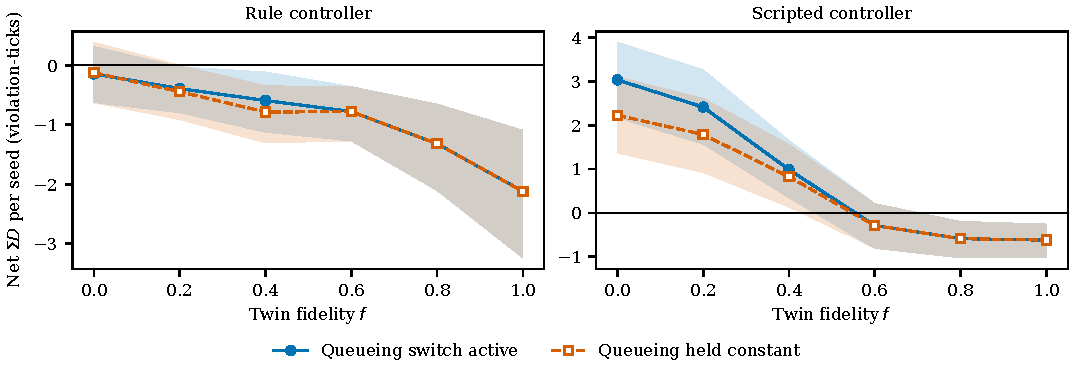
\includegraphics[width=\textwidth]{figures/fig1_net_sum_d.pdf}
\caption{\NetSD{} per seed over approved candidates against twin fidelity, $n=\NSeeds$ seeds. Shaded bands are 95\% seed-bootstrap intervals; solid circles: queueing switch active; dashed squares: queueing held constant. Negative values mean the approved set is locally better than reject-all. Scripted crossing: \ScrCrossI{} \ScrCrossCII{} (switch active), \ScrCrossII{} \ScrCrossCIII{} (held constant).}
\label{fig:netsd}
\end{figure*}
For the scripted controller, \netSD{} falls monotonically from \ScrNetZeroI{} at $f=0$ to \ScrNetTenI{} at $f=1$ and crosses zero at \ScrCrossI{} \ScrCrossCII{} (Fig.~\ref{fig:netsd}). The crossing lies between $f=0.4$ and $f=0.6$, exactly where the queueing switch flips, so as first observed it could not be attributed to fidelity. The crossing only became attributable after the control that holds the queueing model constant: it then sits at \ScrCrossII{} \ScrCrossCIII{}, monotone, with \ScrCrossSingleII{} of \BootResamples{} resamples showing exactly one crossing. The 0.4$\rightarrow$0.6 step in the held-constant condition is \ScrStepFourSixII{} \ScrStepFourSixCIII, while the switch itself is worth only \ScrSwitchFour{} \ScrSwitchFourCI{} per seed at $f=0.4$ ($p=\ScrSwitchFourP$). The rule controller's \netSD{} is at or below zero at every level in both conditions (\RuleNetZeroI{} to \RuleNetTenI), with no crossing; held constant, its curve is flat between 0.4 and 0.6 (\RuleStepFourSixII{} \RuleStepFourSixCIII) and is not fitted through.

\subsection{Episode-level benefit for the rule controller}
\begin{figure}[t]
\centering
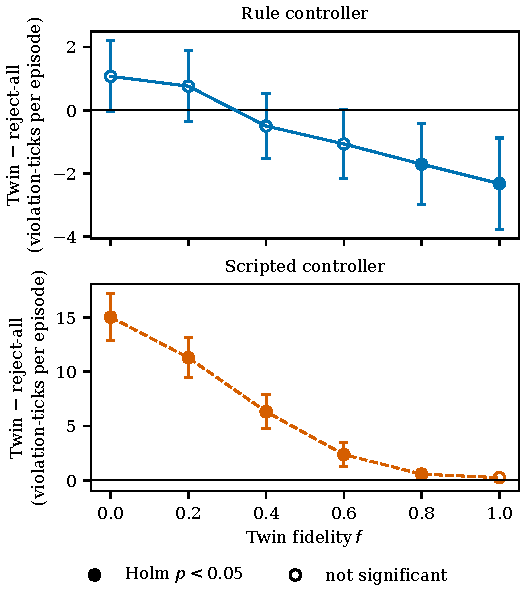
\includegraphics[width=\columnwidth]{figures/fig2_episode_difference.pdf}
\caption{Episode-level difference, twin $-$ reject-all, by fidelity (condition (i), $n=\NSeeds$). Bars are 95\% $t$-intervals; filled markers: Holm $p<0.05$; open markers: not significant. Negative means the twin gate is better.}
\label{fig:episode}
\end{figure}
Only for the rule controller does the twin beat reject-all at the episode level: by \RuleEpTenI{} \RuleEpCITenI{} at fidelity 1.0 (exact Wilcoxon $p=\RuleEpPTenI$, Holm $p=\RuleEpHolmTenI$) and \RuleEpEightI{} \RuleEpCIEightI{} at 0.8 (Holm $p=\RuleEpHolmEightI$), identically in both queueing conditions. The effect is small: about \RuleTenPctBaseline{} of the \RuleRejEpMeanI-tick reject-all baseline. It is concentrated in \RuleEpNZTenI{} of \NSeeds{} seeds (\RuleTenPctSeeds), and \RuleEpWorseTenI{} of those seeds went the wrong way (\RuleEpBetterTenI{} better). The fidelity-1.0 result survives Bonferroni correction across the \BonfFamily{} unique comparisons of both controllers and both conditions (adjusted $p=\BonfRuleTen$); the fidelity-0.8 result does not (adjusted $p=\BonfRuleEight$). The superseded 10-seed estimate for this comparison overstated the effect; all figures here are the \NSeeds-seed values. For the scripted controller, twin@1.0 is not distinguishable from reject-all (\ScrEpTenI{} \ScrEpCITenI, $p=\ScrEpPTenI$, observed power \ScrEpPowerTenI).

\subsection{Classifier quality}
\begin{table}[t]
\centering
\caption{Twin@1.0 as a classifier of harmful actions ($D>\theta$). Scripted: \ScrTTCandidates{} candidates (\ScrTTBeneficial{} beneficial); rule: \RuleTTCandidates{} (\RuleTTBeneficial{} beneficial). FP split into definitional ($\tau<D\le\theta$) and predictive.}
\label{tab:classifier}
\footnotesize
\setlength{\tabcolsep}{2.5pt}
\begin{tabular}{@{}lcrrrrr@{}}
\toprule
Ctrl. & ($\tau,\theta$) & Recall & FPR & Neg. & FP def. & FP pred. \\
\midrule
Scr. & (0,3) & \ScrTTZeroThreeRecall & \ScrTTZeroThreeFPR & \ScrTTZeroThreeNeg & \ScrTTZeroThreeFPDef & \ScrTTZeroThreeFPPred \\
Scr. & (1,1) & \ScrTTOneOneRecall & \ScrTTOneOneFPR & \ScrTTOneOneNeg & \ScrTTOneOneFPDef & \ScrTTOneOneFPPred \\
Scr. & (3,3) & \ScrTTThreeThreeRecall & \ScrTTThreeThreeFPR & \ScrTTThreeThreeNeg & \ScrTTThreeThreeFPDef & \ScrTTThreeThreeFPPred \\
Rule & (0,3) & \RuleTTZeroThreeRecall & \RuleTTZeroThreeFPR & \RuleTTZeroThreeNeg & \RuleTTZeroThreeFPDef & \RuleTTZeroThreeFPPred \\
Rule & (1,1) & \RuleTTOneOneRecall & \RuleTTOneOneFPR & \RuleTTOneOneNeg & \RuleTTOneOneFPDef & \RuleTTOneOneFPPred \\
Rule & (3,3) & \RuleTTThreeThreeRecall & \RuleTTThreeThreeFPR & \RuleTTThreeThreeNeg & \RuleTTThreeThreeFPDef & \RuleTTThreeThreeFPPred \\
\bottomrule
\end{tabular}
\end{table}
\begin{figure}[t]
\centering
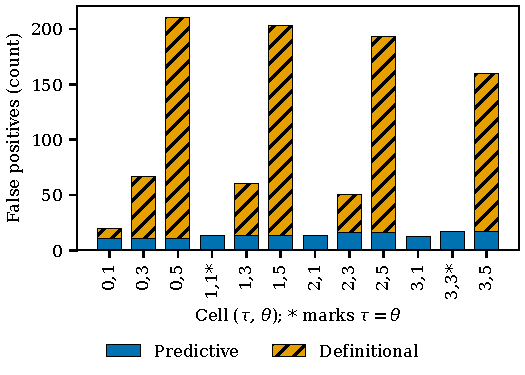
\includegraphics[width=\columnwidth]{figures/fig4_false_positives.pdf}
\caption{False positives of the scripted controller's twin@1.0 across ($\tau,\theta$) cells, split into definitional ($\tau<D\le\theta$) and predictive. The definitional band is empty on the $\tau=\theta$ diagonal (marked *).}
\label{fig:fp}
\end{figure}
\textbf{(a) Reading the classifier on the $\tau=\theta$ diagonal.} At the operating setting $\tau=\GateTau$, $\theta=\HarmTheta$, the scripted twin@1.0 has FPR \ScrTTZeroThreeFPR{} \ScrTTZeroThreeFPRCI{}, but \ScrTTZeroThreeFPDef{} of its \ScrTTZeroThreeFP{} false positives (\ScrTTZeroThreeDefShare) are definitional: actions with $0<D\le\HarmTheta$ that cause real harm below $\theta$. On the diagonal that band is empty by construction, so every false positive is a genuine prediction error. At $\tau=\theta=3$ recall is \ScrTTThreeThreeRecall{} and FPR is \ScrTTThreeThreeFPR{} \ScrTTThreeThreeFPRCI{} (Table~\ref{tab:classifier}, Fig.~\ref{fig:fp}); the rule twin gives FPR \RuleTTOneOneFPR--\RuleTTThreeThreeFPR{} with recall \RuleTTOneOneRecall--\RuleTTThreeThreeRecall. These rates rest on few negatives (\ScrTTThreeThreeNeg{} scripted, \RuleTTThreeThreeNeg{} rule) and, for the rule controller, on \RuleTTCandidates{} candidates in total; they describe a good filter on these candidates, not a general classifier.

\textbf{(b) The operating point.} The diagonal is where the classifier is read, not where the gate should run. At $\tau=3$ the scripted gate's \netSD{} turns positive, \ScrTTThreeThreeNet{} \ScrTTThreeThreeNetCI{}, against \ScrTTZeroThreeNet{} \ScrTTZeroThreeNetCI{} at $\tau=0$, because a tolerance of 3 admits harmful scale-ups. The $\tau>0$ rows relabel a fixed corpus of decisions taken at $\tau=0$; they do not simulate a system running at $\tau>0$.

\subsection{The benefit ceiling}
\begin{figure}[t]
\centering
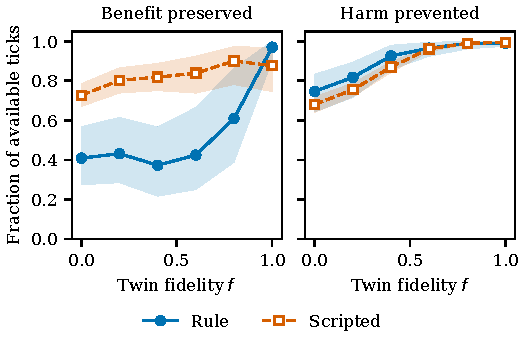
\includegraphics[width=\columnwidth]{figures/fig3_benefit_harm.pdf}
\caption{Benefit preserved and harm prevented against twin fidelity (condition (i), $n=\NSeeds$), with 95\% seed-bootstrap intervals.}
\label{fig:bphp}
\end{figure}
A gate cannot beat reject-all by more than the benefit reject-all discards. On the reject-all trajectory that benefit is \RuleRejAvailBenefitI{} violation-ticks (\RuleRejAvailBenefitPerSeedI{} per seed) in \RuleRejSeedsBenefitI{} of \NSeeds{} seeds for the rule controller, and \ScrRejAvailBenefitI{} ticks (\ScrRejAvailBenefitPerSeedI{} per seed) in \ScrRejSeedsBenefitI{} seeds for the scripted controller, where reject-all's trajectory holds \ScrRejBeneficialI{} beneficial against \ScrRejHarmfulAboveThreeI{} harmful scale-ups. Seeds with any beneficial candidate in any arm number \RuleAnyArmSeedsBenefitI{} (rule) and \ScrAnyArmSeedsBenefitI{} (scripted), but most of that benefit exists only on trajectories that earlier actions created. Harm prevented rises with fidelity for both controllers; benefit preserved for the rule controller is flat up to 0.6 and rises only at 0.8--1.0 (Fig.~\ref{fig:bphp}). The scripted null at fidelity 1.0 is therefore structural.

\subsection{Live-model descriptive study}
\begin{figure}[t]
\centering
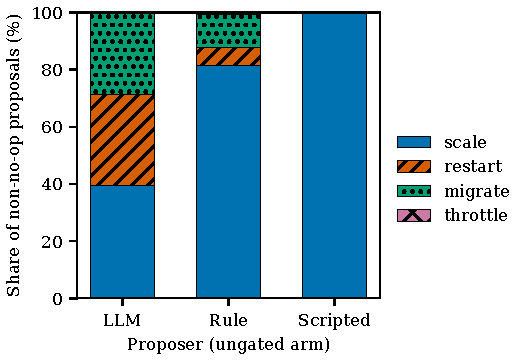
\includegraphics[width=\columnwidth]{figures/fig5_action_mix.pdf}
\caption{Action-type mix of non-no-op proposals on the ungated arm: live model (\LLMSeeds{} seeds), rule and scripted controllers (\NSeeds{} seeds).}
\label{fig:mix}
\end{figure}
\begin{figure}[t]
\centering
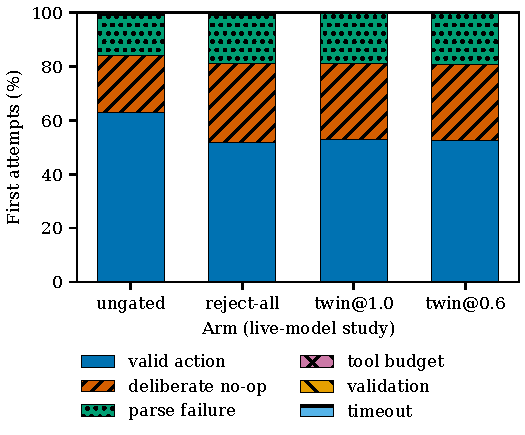
\includegraphics[width=\columnwidth]{figures/fig6_llm_outcomes.pdf}
\caption{Live-model first-attempt outcome at each scheduled decision, by arm (\LLMSeeds{} seeds, \LLMUngatedFirstN{} first attempts per arm).}
\label{fig:outcomes}
\end{figure}
A hosted model (\LLMModel, temperature \LLMTemperature, one prompt) was run as a proposer on \LLMSeeds{} seeds with ungated, reject-all, twin@1.0 and twin@0.6 arms. This study is descriptive. Valid non-no-op first proposals occurred at \LLMProducedMin--\LLMProducedMax{} of scheduled decisions, and final parse failures at \LLMParseMin--\LLMParseMax{}, each resolved to an explicit no-op fallback (Fig.~\ref{fig:outcomes}). The model's action mix differs from both baselines: on the ungated arm \LLMUngatedMixScale{} scale, \LLMUngatedMixRestart{} restart and \LLMUngatedMixMigrate{} migrate, against \RuleUngatedMixScale{} scale for the rule controller and \ScrUngatedMixScale{} for the scripted one (Fig.~\ref{fig:mix}). Recoverable benefit on the reject-all trajectory is \LLMRejectAvailBenefit{} ticks, \LLMRejectAvailBenefitPerSeed{} per seed in \LLMRejectSeedsBenefit{} of \LLMSeeds{} seeds, larger per seed than for either baseline. The paired twin@1.0 $-$ reject-all difference, \LLMTwinTenMean{} \LLMTwinTenCI{} (exact Wilcoxon $p=\LLMTwinTenP$, Holm $p=\LLMTwinTenHolm$, observed power \LLMTwinTenPower), is an underpowered pilot statistic; no episode-level effect is claimed.

\subsection{Local counterfactuals do not compose into episode effects}
\NetSD{} is a sum of \Horizon-tick counterfactuals with a no-op continuation, and it does not add up to closed-loop episode effects. For the scripted controller at fidelity 1.0, \netSD{} is \ScrNetTenI{} per seed, predicting a twin advantage, while the episode difference is \ScrEpTenI: the sign is wrong. The scripted \netSD{} crossing near \ScrCrossI{} has no episode-level counterpart; the episode curve approaches zero from above and never crosses. The mechanism is visible in single seeds of the earlier \SignAblationSeeds-seed ablation runs, cited here as worked examples and not as effect estimates: on seed \SignSeed, approved scale-ups summed to \SignPredicted{} locally, but the episode ended \SignObserved{} ticks worse than reject-all, because approved scale-ups alter later states that the no-op continuation does not represent. For the rule controller the sign is right but migrations are underestimated: on seed \MigImmuneSeed{} of the gateway-exposed ablation the observed episode effect was \MigImmuneRatio{}$\times$ the local sum with the gateway immune (\MigImmunePredicted{} predicted, \MigImmuneObserved{} observed) and \MigFaultableRatio{}$\times$ with the gateway faultable (\MigFaultablePredicted{} predicted, \MigFaultableObserved{} observed), because a migration's downtime is paid inside the horizon while its benefit accrues for the rest of the fault. Local metrics describe the filter; performance claims need episode outcomes.

\section{Threats to Validity}
\textbf{Shared simulator code.} The twin and the labeller are forks of the same simulator, so model-structure error is represented only through the five degradation axes; fidelity 1.0 is a harness sanity check, not an attainable twin. \textbf{Relabelled corpus.} The $\tau>0$ rows relabel decisions taken at $\tau=0$. \textbf{Shared response cache.} In the live study one response cache served all arms, so arms reuse identical responses for identical prompts, and which arm first queries the model depends on execution order. \textbf{Synthetic only.} All results come from a synthetic simulator; no numerical comparison with systems evaluated on real replicas is meaningful. \textbf{Incomplete cost accounting.} The historical live study retained input and visible-output tokens but not thinking tokens or failed-request usage; its rate-card figure (\$\LLMRateCardCost{} for \LLMBilledCalls{} billed calls) is not an invoice.

\section{Limitations and Future Work}
The live-model evidence is a single model, prompt and cache realisation at \LLMSeeds{} seeds. The normal-approximation requirement computed from the \LLMSeeds-seed data is $n=\LLMTwinTenNeed$ seeds for 80\% power on the twin@1.0 $-$ reject-all comparison; a \LLMTwinTenNeed-seed live-model confirmation run is scheduled. A design with more restart and migration opportunities per episode would raise the benefit ceiling more efficiently than more seeds.

\section{Conclusion}
Comparing a twin gate with reject-all on counterfactually labelled proposals separates what the twin predicts from what it blocks. On \NSeeds{} seeds the twin's value depends strongly on fidelity: low fidelity is worse than no gate, and the net local benefit crosses zero near \ScrCrossII{} once the queueing model is held constant. The episode-level gain is real for one controller, small, and concentrated in a few seeds, bounded by the benefit reject-all discards. Local counterfactual metrics are useful for describing the filter but do not compose into episode effects.

\bibliographystyle{IEEEtran}
\bibliography{refs}

\end{document}
